% PREPARAÇÃO DO DATASET -------------------------------------------

\section{Preparação dos dados}
\label{sec:metodologia-preparacao-dados}

Para tornar as amostras do ASL-Phono compatíveis com a entrada dos modelos que serão utilizados mais adiante, aplicamos uma transformação simples que consiste em codificar seus atributos fonológicos como blocos ou ``palavras'' únicas, mais compactas. Ou seja, ao invés de utilizar como entrada sequências de frames que contêm propriedades aninhadas, adotamos aqui sequências de blocos compactos que codificam a mesma informação de uma forma mais amigável a modelos sequenciais.

Observe na \autoref{tab:codificacao-bloco} um exemplo deste processo. Na primeira linha, temos os valores originais das propriedades providas para o frame de uma amostra do ASL-Phono; na segunda linha, geram-se acrônimos a partir desses atributos para realizar uma primeira compactação -- mas que não é um passo necessariamente obrigatório; na terceira linha, temos um bloco ou palavra única gerada pela composição desses acrônimos; finalmente, na última linha, temos o exemplo de uma sequência desses blocos.

% Please add the following required packages to your document preamble:
% \usepackage{graphicx}
% \usepackage[table,xcdraw]{xcolor}
% If you use beamer only pass "xcolor=table" option, i.e. \documentclass[xcolor=table]{beamer}
\begin{table}[ht!]
    \centering
    \caption{Exemplo de compactação dos atributos fonológicos do frame de uma amostra do ASL-Phono em uma ``palavra''.}
    \label{tab:codificacao-bloco}
    \resizebox{0.95\textwidth}{!}{%
        \begin{tabular}{r|cccccc}
            \hline
            \rowcolor[HTML]{EFEFEF}
            \multicolumn{1}{l|}{\cellcolor[HTML]{EFEFEF}} & \multicolumn{6}{c}{\cellcolor[HTML]{EFEFEF}Atributos}                                                                                                                                                                                                                          \\ \cline{2-7}
            \rowcolor[HTML]{EFEFEF}
                                                          & \multicolumn{3}{c|}{\cellcolor[HTML]{EFEFEF}Mão dominante}                    & \multicolumn{3}{c}{\cellcolor[HTML]{EFEFEF}Mão não-dominante}                                                                                                                                  \\
            \rowcolor[HTML]{EFEFEF}
                                                          & Movimento                                                                     & Orientação                                                    & \multicolumn{1}{c|}{\cellcolor[HTML]{EFEFEF}Config. mão} & Movimento                  & Orientação           & Config. mão     \\ \hline
            Valores originais                             & \textit{right\_up}                                                            & \textit{left}                                                 & \multicolumn{1}{c|}{\textit{bentBL}}                     & \textit{left\_front\_down} & \textit{back\_right} & \textit{bentBL} \\
            Valores abreviados                            & \textit{ru}                                                                   & \textit{l}                                                    & \multicolumn{1}{c|}{\textit{bentBL}}                     & \textit{lfd}               & \textit{br}          & \textit{bentBL} \\ \hline
            {\color[HTML]{3531FF} Palavra}                & \multicolumn{6}{c}{{\color[HTML]{3531FF} \textit{ru-l-bentBL-lfd-br-bentBL}}}                                                                                                                                                                                                  \\ \hline
        \end{tabular}%
    }
    \nomefonte{}
\end{table}


% RESAMPLING DO DATASET -------------------------------------------

Conforme observa-se pela \autoref{tab:dataset-phono-stats}, o ASL-Phono apresenta um desbalanceamento no número de amostras disponíveis por sinal. Em média, há 3,68 amostras disponíveis por sinal porém, enquanto alguns sinais têm apenas 1 amostra, outros apresentam um número atípico de 59. Isso poderia influenciar o desempenho dos modelos utilizados adiante, uma vez que durante o treinamento alguns sinais seriam favorecidos e, outros, penalizados. 

Por conta disso, aplicamos dois procedimentos para reduzir o desbalanceamento desses dados: primeiro, eliminamos os sinais com apenas 1 amostra, uma vez que esse número é insuficiente para que o modelo seja capaz de aprender e generalizar acerca desses sinais, sobretudo quando o \textit{dataset} é particionado durante o treinamento; segundo, realizamos uma reamostragem do \textit{dataset} para equilibrar o número de amostras.

Observe na \autoref{subfig:dataset-resampling-antes} um perfil detalhado dos dados antes da reamostragem. É possível perceber que o número de amostras é bastante disperso pelo eixo horizontal do gráfico: por exemplo, 726 sinais apresentam 2 amostras disponíveis; seguidos por 552 sinais com 4 amostras; mas, no outro extremo, temos que apenas um número muito pequeno de sinais (entre 1 e 3) apresentam um grande número de amostras disponíveis (entre 13 e 59), respectivamente.

\begin{figure}[ht!]
    \centering
    \caption{
        \textmd{Número de amostras disponíveis por sinal (\subref{subfig:dataset-resampling-antes}) antes da reamostragem e (\subref{subfig:dataset-resampling-depois}) após a reamostragem do ASL-Phono. Por exemplo, lê-se que 726 sinais possuem 2 amostras disponíveis antes da reamostragem.}
    }
    \subcaptionbox{\label{subfig:dataset-resampling-antes}}{
        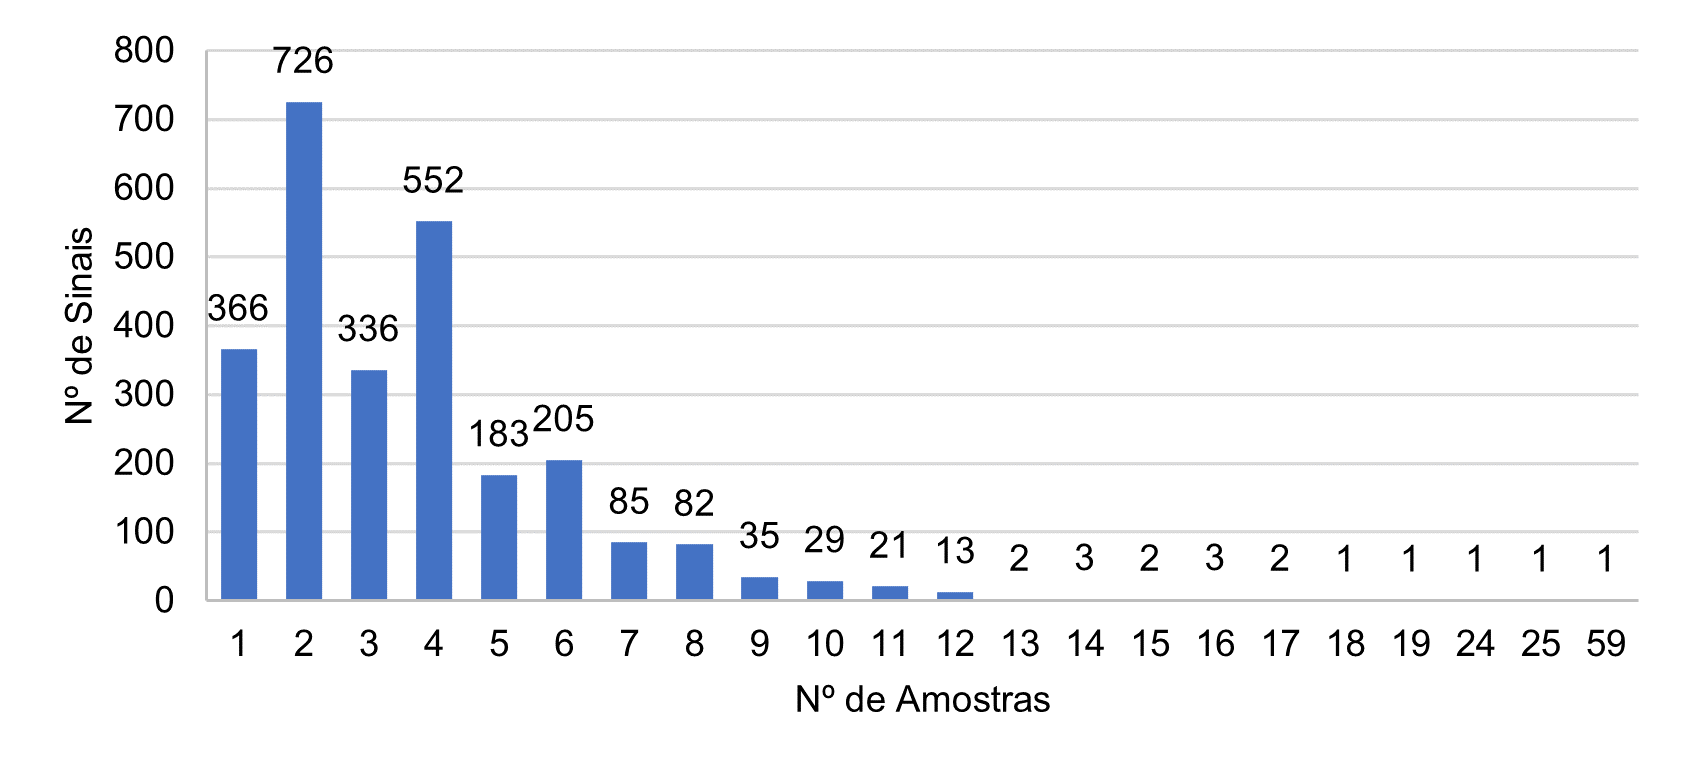
\includegraphics[height=6cm]{capitulos/metodologia/imagens/dataset_resampling_antes}
    }%
    \hspace{1cm}
    \subcaptionbox{\label{subfig:dataset-resampling-depois}}{
        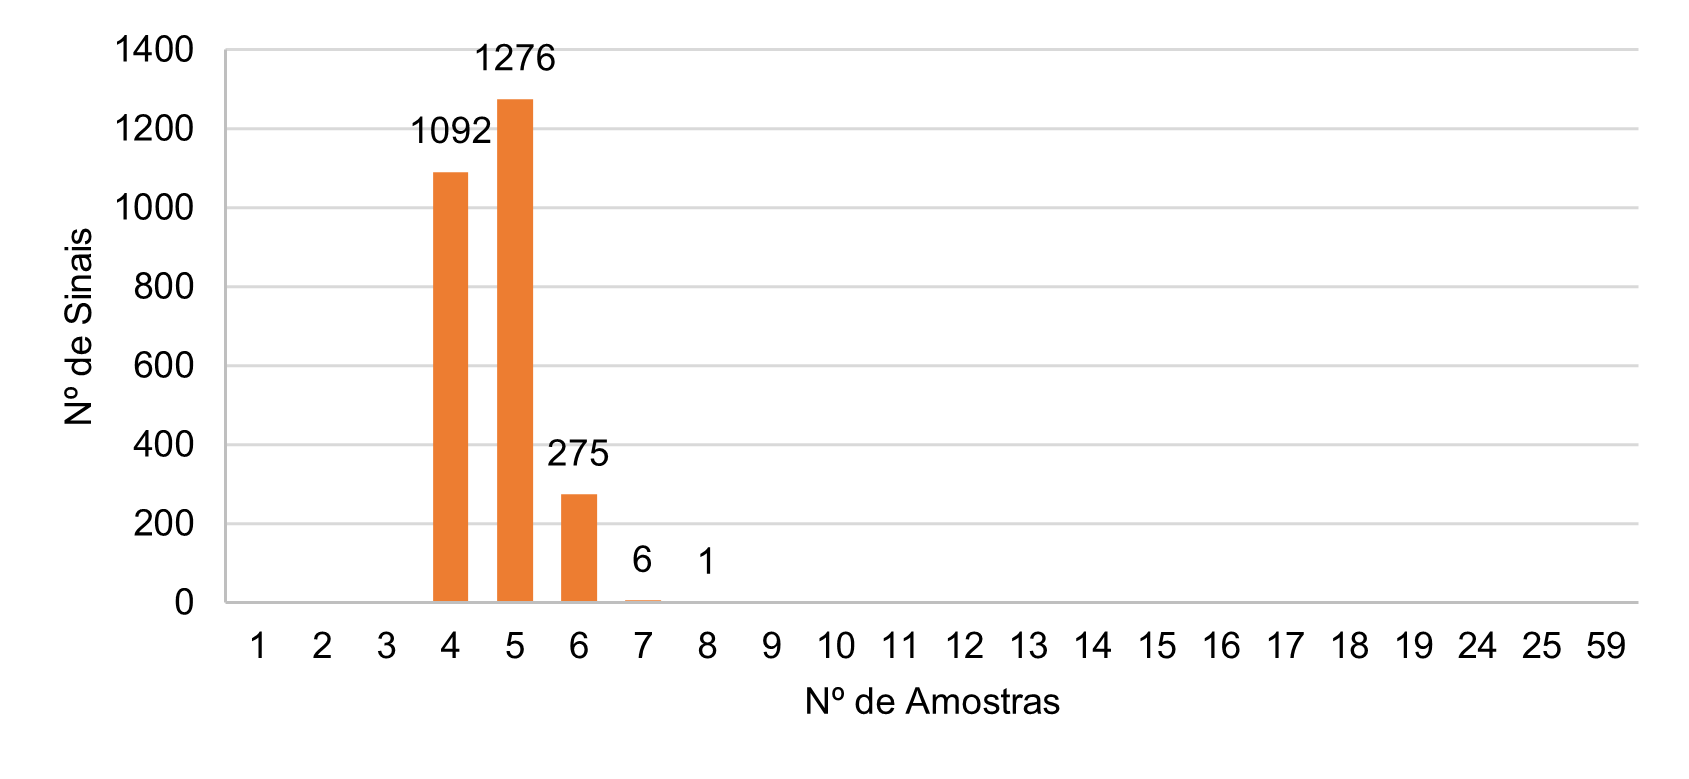
\includegraphics[height=6cm]{capitulos/metodologia/imagens/dataset_resampling_depois}
    }%
    \nomefonte{}
    \label{fig:dataset-resampling}
\end{figure}

Aplicamos então uma reamostragem \textit{naive random under-sampling} (ou sub-amostragem aleatória ingênua, que reduz o número de amostras através de uma seleção aleatória de algumas delas para os sinais que estão super-representados) seguida de uma \textit{naive random over-sampling} (ou sobre-amostragem aleatória ingênua, que replica aleatoriamente algumas das amostras existentes para os sinais que estão sub-representados).
Para estabelecer o novo número de amostras por sinal \(x'\), utilizamos a \autoref{eqn:resampling-target}: 

\begin{equation}
    \label{eqn:resampling-target}
    x' = round( \overline{a} + \ln(x) )
\end{equation}

Onde \(\overline{a}\) refere-se ao número médio de amostras por sinal no \textit{dataset} e \(x\) é o número de amostras para aquele sinal. Observe na \autoref{subfig:dataset-resampling-depois} como os dados ficaram organizados após a reamostragem. Em resumo, a equação faz com que o número de amostras por sinal se concentre mais uniformemente a partir do valor da média.
